\documentclass[a4paper]{article}
\usepackage{fullpage, graphicx}

\begin{document}
\title{G52SOF - Vision and Scope Document}
\author{Harry Coupe, PSYHC5, 4321806}
\maketitle
\pagebreak


\section*{\underline{1.1 Background}}
The goal behind this project is to develop and release an app directed at students who, in the present day,
suffer from extremely high levels of stress and anxiety. This is due to expectations and sheer amount of work they deal
with during assessment periods and exams. The app we plan to develop will be designed to aid students in dealing with this
stress in their everyday lives and will include multiple features. Apps which are designed to aid with mental health and well-being do exist on many app stores. Currently however, there are not any which are designed specifically to help students with their assessments.. A university well-being team has commissioned us to create such an android mobile app for their students. They have noticed the trend of rising stress and wish for a way their students can easily manage their deadlines and stress levels.

Whilst mental health apps have been on the rise in recent years, as stated before, a clear gap in the market has been noted with the apparent lack of a good option for students who require this assistance in an easy to use application. As well as this gap in the market we have a user base that can be used for testing and marketing the app to at a later date, as well as with the well-being team commissioning the app.


\section*{\underline{1.2 Business Opportunity}}
As described before there is an opening in the market that has been identified and we have been commissioned to fill it. Currently, many mental and physical self-help apps exist, as well as organisation apps which assist with managing deadlines. Neither of these combine the two themes, nor are they aimed specifically at our target audience: students. By addressing this gap, not only do we allow ourselves minimal competitors early on due to being the only app competently combining the two categories into a simple and easy to use app. 
What we will be developing is an android application that will allow students to organise and manage deadlines in a simple manner on a calendar. Other features will include access to exercises to aid with stress and advice on how to deal with the aforementioned issues they deal with.   


\section*{\underline{1.3 Business Objectives}}
\begin{tabular}{|c|c|}
\hline
\textbf{Financial} & \textbf{Non-Financial} \\
\hline
Achieve a 5\% return on investment & Gain 30\% of the university's student body as users\\
\hline
Capture 10\% of market share in 12 months & Gain university's student unions support of the app\\
\hline
 & Retain 80-90\% of that initial 30\% user base\\
\hline
 & Be in the top 30 of the apps category on the app store\\
\hline
\end{tabular}

\section*{\underline{1.4 Success Metrics}}
These metrics are used to judge and measure the continuing success of the project as it develops over time.
\begin{itemize}
	\item The application itself will be completed within 4 months
	\item From a survey of students using the app we will have a satisfaction level of 90\% average or above
	\item From a survey of students using the app they will confirm to feel the app has helped deal with assessment stress
	\item An increase in productivity and grades of 10\% from before to after using the app
\end{itemize}
\pagebreak


\section*{\underline{1.5 Vision Statement}}
For students who suffer from school related stress, the “Exam and Assessment Management app” is an app that can help students manage deadlines, and this combines that with helpful exercises and advice on maintaining mental and physical well-being through stressful assessment periods. Unlike other mental health apps, which do not target students specifically, our product can aid students with their specific needs, as well as with their wider mental and physical health issues.

\section*{\underline{1.6 Business Risks}}
There are several business risks involved in developing an app, A list of these initial positive and negative risks will be detailed below.\\
\textbf{{\large Positive:}}
\begin{itemize}
	\item Risk of not developing is students stress and anxiety continue to grow in exam periods with no developed ways of aiding them without our app
	\item Not developing would risk missing a gap in the market with minimal competition as of right now
\end{itemize}
\textbf{{\large Negative:}}
\begin{itemize}
	\item A risk of developing this app is getting people to install a new app is inherently difficult so adoption is not guaranteed
	\item Between now and release someone could have also noticed the gap in the market we are aimed at and beat us to release
	\item Students do not find the app helpful and user retention is extremely low
\end{itemize}

\section*{\underline{1.7 Business Assumptions}}
\begin{itemize}
	\item The well-being staff will be able to gain interest and help from the student body for:
	\begin{itemize}
		\item Testing
		\item Surveying
		\item Marketing
	\end{itemize}
	\item Students actually feel a need for this sort of app and that it will be useful to them
	\item A concurrent user-base of 500 to sustain revenue
\end{itemize}
\pagebreak


\section*{\underline{2.1 Major Feature Description}}
\begin{itemize}
	\item A calendar for use with planning deadlines and exam dates
	\begin{itemize}
		\item This calendar should be able to be imported/used with other apps such as google calendar.
		\item Items put in should have the ability to be set as alerts on the users phone.
		\item User should be able to set intermediate deadlines for having parts of projects finished with the same functionality of a normal deadline
		\item Teachers should be able to set students deadlines onto this calendar providing the account was make with a student email address
	\end{itemize}
	
	\item A list of available and suggested exercises for students to use to help deal with stressful periods
	\begin{itemize}
		\item The exercises on here should cover a wide range of potential users and come from trusted sources.
		\item Trusted sources and users should be able to upload and edit exercises to keep the information contained within the app evolving.
		\item A rating system will allow users to show how useful or not exercises may be to keep information relevant and helpful to users.
	\end{itemize}
	
	\item Access to advice on how to deal with assessment stress and anxiety
	\begin{itemize}
		\item A forum/message board system where students in similar situations can share experiences and help
		\item A live-chat/email system with student well-being teams to help with crises where fast response and help is available
		\item Contacts to external organisations who help people in issues of mental and physical health
	\end{itemize}		
\end{itemize}

\section*{\underline{2.2 Scoping Out Initial Release}}
This will be the simplest working version of the app we plan to make. All it must show is the core functionality that is required to show the vision of the project. This functionality would be:
\begin{itemize}
	\item A working calendar that can have events/deadlines/assessments added to it
	\item A view for showing exercises for students to use to help deal with stressful periods
	\item A view for accessing advice on how to deal with assessment stress and anxiety
\end{itemize}

This version 0.1 will be completed a month after the initial prototype is finalised. 
\pagebreak

\section*{\underline{2.3 Scope of Subsequent Releases}}
Figure 1 below shows the feature tree of the planned app. This is the final functionality each main section of the app should contain by completion. As stated before this planned tree will be completed within 4 months of the initial prototypes approval.

\begin{figure}[h!]
	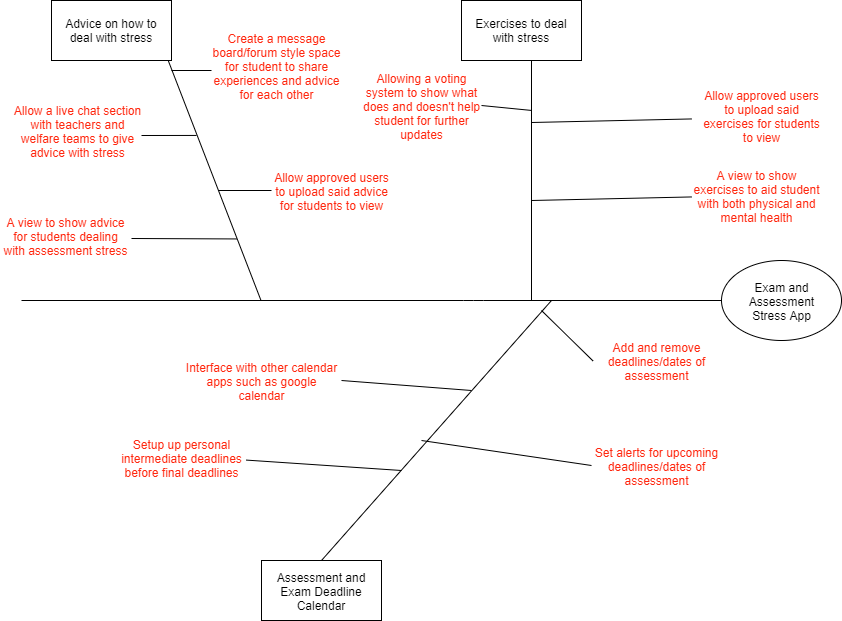
\includegraphics[scale=0.5]{FeatureTree.png}
	\caption{Feature Tree of the app}
	\label{fig:FeatureTree}
\end{figure}

\pagebreak
\section*{\underline{3.1 Describing Stakeholder Profiles}}
\textbf{Well-Being Team}
The major value on benefit to this stakeholder is:
\begin{itemize}
	\item Will help them interact with and aid their students on a regular basis
	\item Give them a consistent space to update with advice and help where students know it will be
	\item Easy way to engage with students who need their help
\end{itemize}

\noindent\textbf{Students}
The major value on benefit to this stakeholder is:
\begin{itemize}
	\item Easy to use place to organise many deadlines
	\item Easy access to help and advice on how to deal with their situations
	\item A potential raise in grades with improved organisation and stress handling
\end{itemize}

\noindent\textbf{Trusted Users}
The major value on benefit to this stakeholder is:
\begin{itemize}
	\item Provide helpful exercises and advice to stressed students
	\item Expand their reach and network with an easy interaction with students
	\item Potential to expand further than without using our user-base 
\end{itemize}

\section*{\underline{3.2 Project Priorities}}
\textbf{Features}
\begin{itemize}
	\item Constraint: With development plan being 4 months features are limited due to fast turn around
	\item Driver: Having adequate features to allow students to manage deadlines and stress
	\item Degree of Freedom: Providing changes and additions are within time and cost scope freedom is there and encouraged
\end{itemize}

\noindent\textbf{Quality}
\begin{itemize}
	\item Constraint: Again time and cost are a big constraint but we will aim for a good balance between amount of features and quality
	\item Driver: Students should have access to quality tools if they search out and decide to use our app
	\item Degree of Freedom: Quality should be a top concern rather than adding more lower quality features 
\end{itemize}

\noindent\textbf{Schedule}
\begin{itemize}
	\item Constraint: Having the app completed to our standards of quality and feature rich in the time scale
	\item Driver: Have the app completed 4 months after prototype approval
	\item Degree of Freedom: The schedule is fairly inflexible
\end{itemize}

\noindent\textbf{Cost}
\begin{itemize}
	\item Constraint: Keeping cost low is essential on a fast turn around product with a small team
	\item Driver: To maximise profits whilst delivering a quality satisfying product
	\item Degree of Freedom: Low freedom with cost and schedule
\end{itemize}

\noindent\textbf{People}
\begin{itemize}
	\item Constraint: Small team of people to keep cost low and people management simple
	\item Driver: Keep small team happy whilst delivering a quality satisfying product
	\item Degree of Freedom: The team is set as is
\end{itemize}
\pagebreak

\section*{\underline{3.3 Deployment Considerations}}
The apps frontend will developed in React, Facebook's JavaScript library. For the back-end Node.js will be used as a modern and widely used back-end language. The system will be built with future maintenance and extensibility in mind by making the most use of Reacts components system to keep code small and reusable throughout. A long side this all code will be put through continuous integration at time of push so all code in repositories passes our quality control.
\end{document}